%\chapter{Schrotrauschen}

%\FloatBarrier
%\begin{figure}[htbp]
%    \centering
%    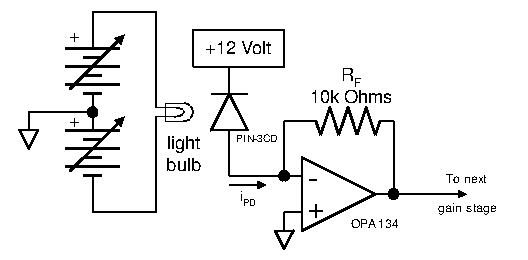
\includegraphics[width=0.5\textwidth]{figs/schrot schaltung.png}
%    \caption{Schaltung fur die LLE-Box zur Beobachtung des Schrotrauschens \cite{praktikum}}
%    \label{fig:schrotschaltung }
%\end{figure}
%\FloatBarrier

%\FloatBarrier
%\begin{figure}[htbp]
%    \centering
%    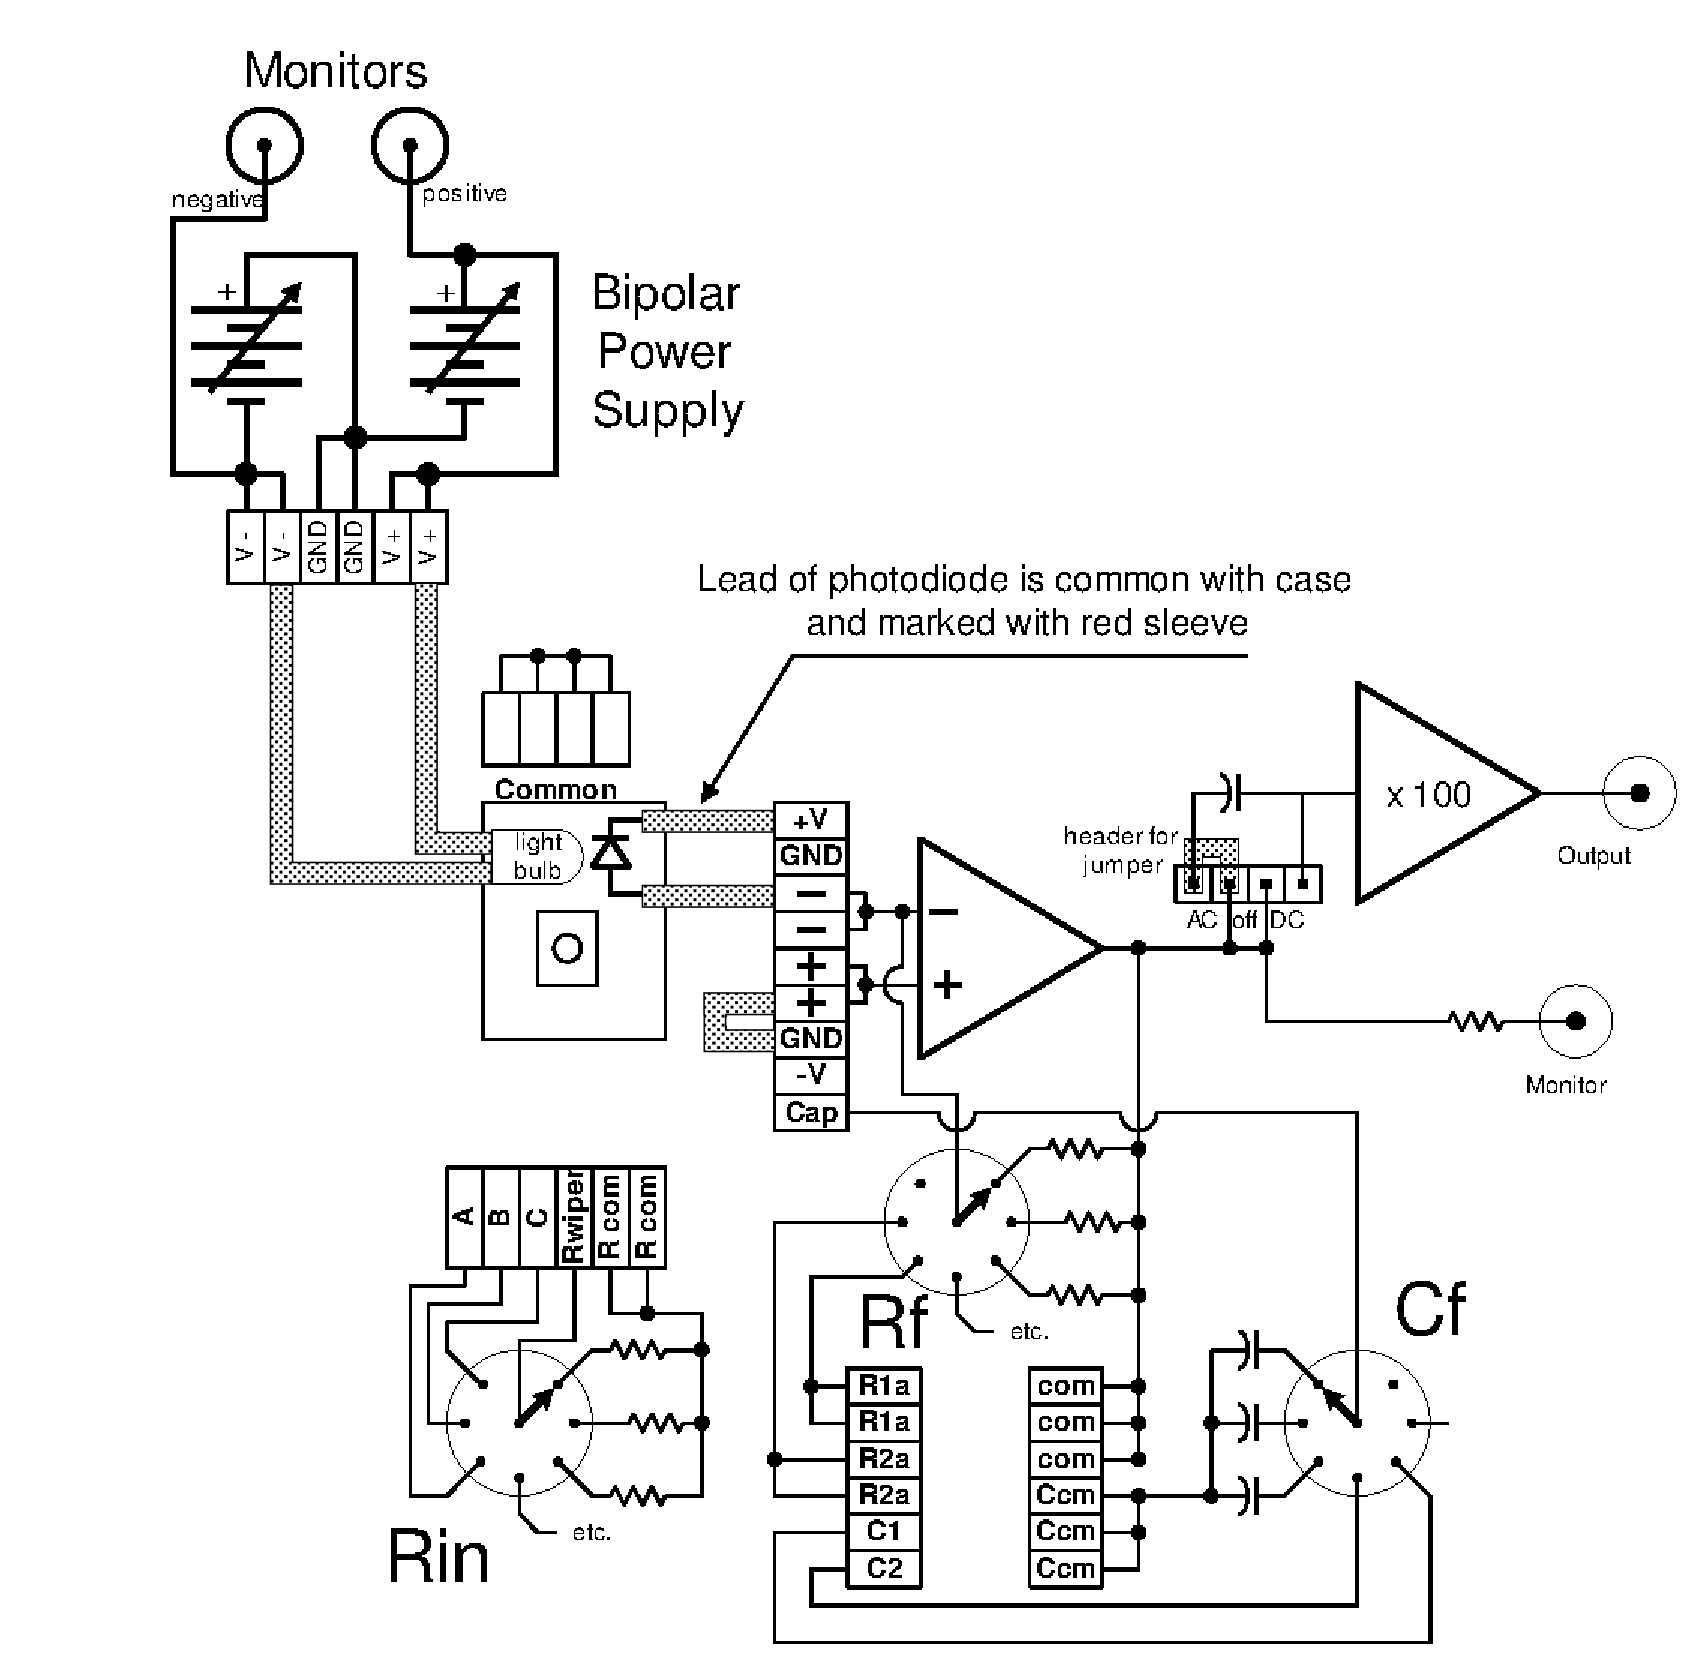
\includegraphics[width=0.5\textwidth]{figs/schrot lle.png}
%    \caption{Interner Schaltplan der LLE-Box zur Beobachtung des Schrotrauschens \cite{praktikum}}
%    \label{fig:schrotlle}
%\end{figure}
%\FloatBarrier

%\section{Beobachten des Schrotrauschens}
%\FloatBarrier
%\begin{figure}[htbp]
%    \centering 
%    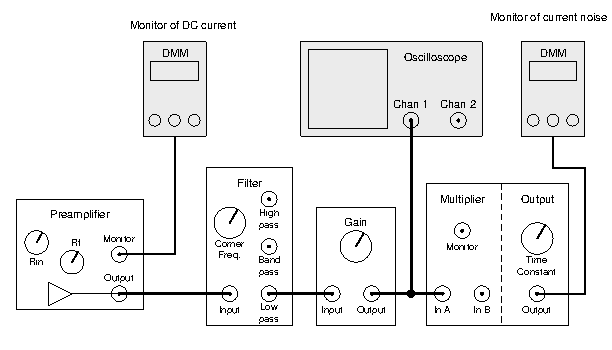
\includegraphics[width=0.5\textwidth]{figs/schrot hle.png}
%  \caption{Schaltung der HLE-Box zur Beobachtung des Schrotrauschens \cite{praktikum}}
 %   \label{fig:schrothle}
%\end{figure}
%\FloatBarrier

%

\section{Schrotrauschen}

Schrotrauschen entsteht aufgrund der diskreten Natur elektrischer Ladungsträger. 
Es tritt immer dann auf, wenn ein elektrischer Strom nicht kontinuierlich, sondern durch eine endliche Zahl unkorrelierter Elektronen fließt. 
In diesem Versuchsteil wird ein solcher Elektronenstrom durch den Photoeffekt erzeugt: Eine Glühlampe emittiert thermische Photonen, die auf eine Photodiode treffen. 
Dort lösen sie über den äußeren Photoeffekt Elektronen aus, die zum beobachtbaren Photostrom beitragen.

Da die Elektronen zufällig eintreffen, folgen die Stromfluktuationen einer Poisson-Verteilung. 
Diese Fluktuationen lassen sich über die Schottky-Formel quantifizieren:

\begin{equation}
    \overline{\delta i^2} = 2 e i_{\text{dc}} \Delta f
    \label{Schottky}
\end{equation}

Dabei bezeichnen:
\begin{itemize}
    \item \( \delta i^2 \): mittlere quadratische Stromschwankung [A\textsuperscript{2}].
    \item \( e \): Elementarladung (\( \approx 1{.}602 \times 10^{-19} \, \si{C} \)), experimentell zu bestimmen.
    \item \( i_{\text{dc}} \): Mittelwert des Gleichstroms (Photostrom).
    \item \( \Delta f \): effektive Bandbreite des Messsystems, siehe Gleichung \ref{eq:bandbreite} (wie in \cref{effektive Bandbreite}).
\end{itemize}

Die effektive Bandbreite ergibt sich aus dem Frequenzgang der verwendeten Filter:

\begin{equation}
    \Delta f = \int_0^\infty G(f)^2 \, df
    \label{eq:bandbreite}
\end{equation}

mit der Verstärkungsfunktion des verwendeten Tiefpassfilters:

\begin{equation}
    G(f) = \left( 1 + \left( \frac{f}{f_l} \right)^4 \right)^{-1/2}
\end{equation}

Der Versuchsaufbau zur Erzeugung des Photostroms ist in Abbildung \ref{fig:schrotschaltung} dargestellt. 
Eine einstellbare Spannungsquelle versorgt eine Glühlampe, deren Licht eine Photodiode bestrahlt und dort über den Photoeffekt einen Gleichstrom \( i_{\text{dc}} \) erzeugt.

\FloatBarrier
\begin{figure}[htbp]
    \centering
    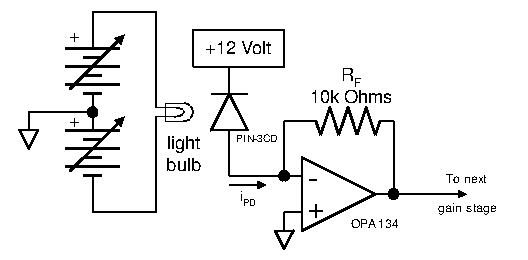
\includegraphics[width=0.5\textwidth]{figs/schrot schaltung.png}
    \caption{Versuchsaufbau zur Erzeugung des Photostroms mittels Glühlampe und Photodiode \cite{praktikum}}
    \label{fig:schrotschaltung}
\end{figure}
\FloatBarrier

Die Photodiode ist über einen invertierenden Verstärker (LLE-Box) mit einem Rückkopplungswiderstand \( R_f = \SI{10}{\kilo\ohm} \) verschaltet. Der resultierende Photostrom erzeugt eine proportionale Spannung:

\begin{equation}
    V_{\text{monitor}} = - R_f \cdot i_{\text{dc}}, \qquad \Delta V_{\text{monitor}} = R_f \cdot \Delta i_{\text{dc}}
\end{equation}

Die vollständige Signalverarbeitung ist in Abbildung \ref{fig:schrotboxes} dargestellt.

\FloatBarrier
\begin{figure}[htbp]
    \centering
    \begin{subfigure}[t]{0.48\textwidth}
        \centering
        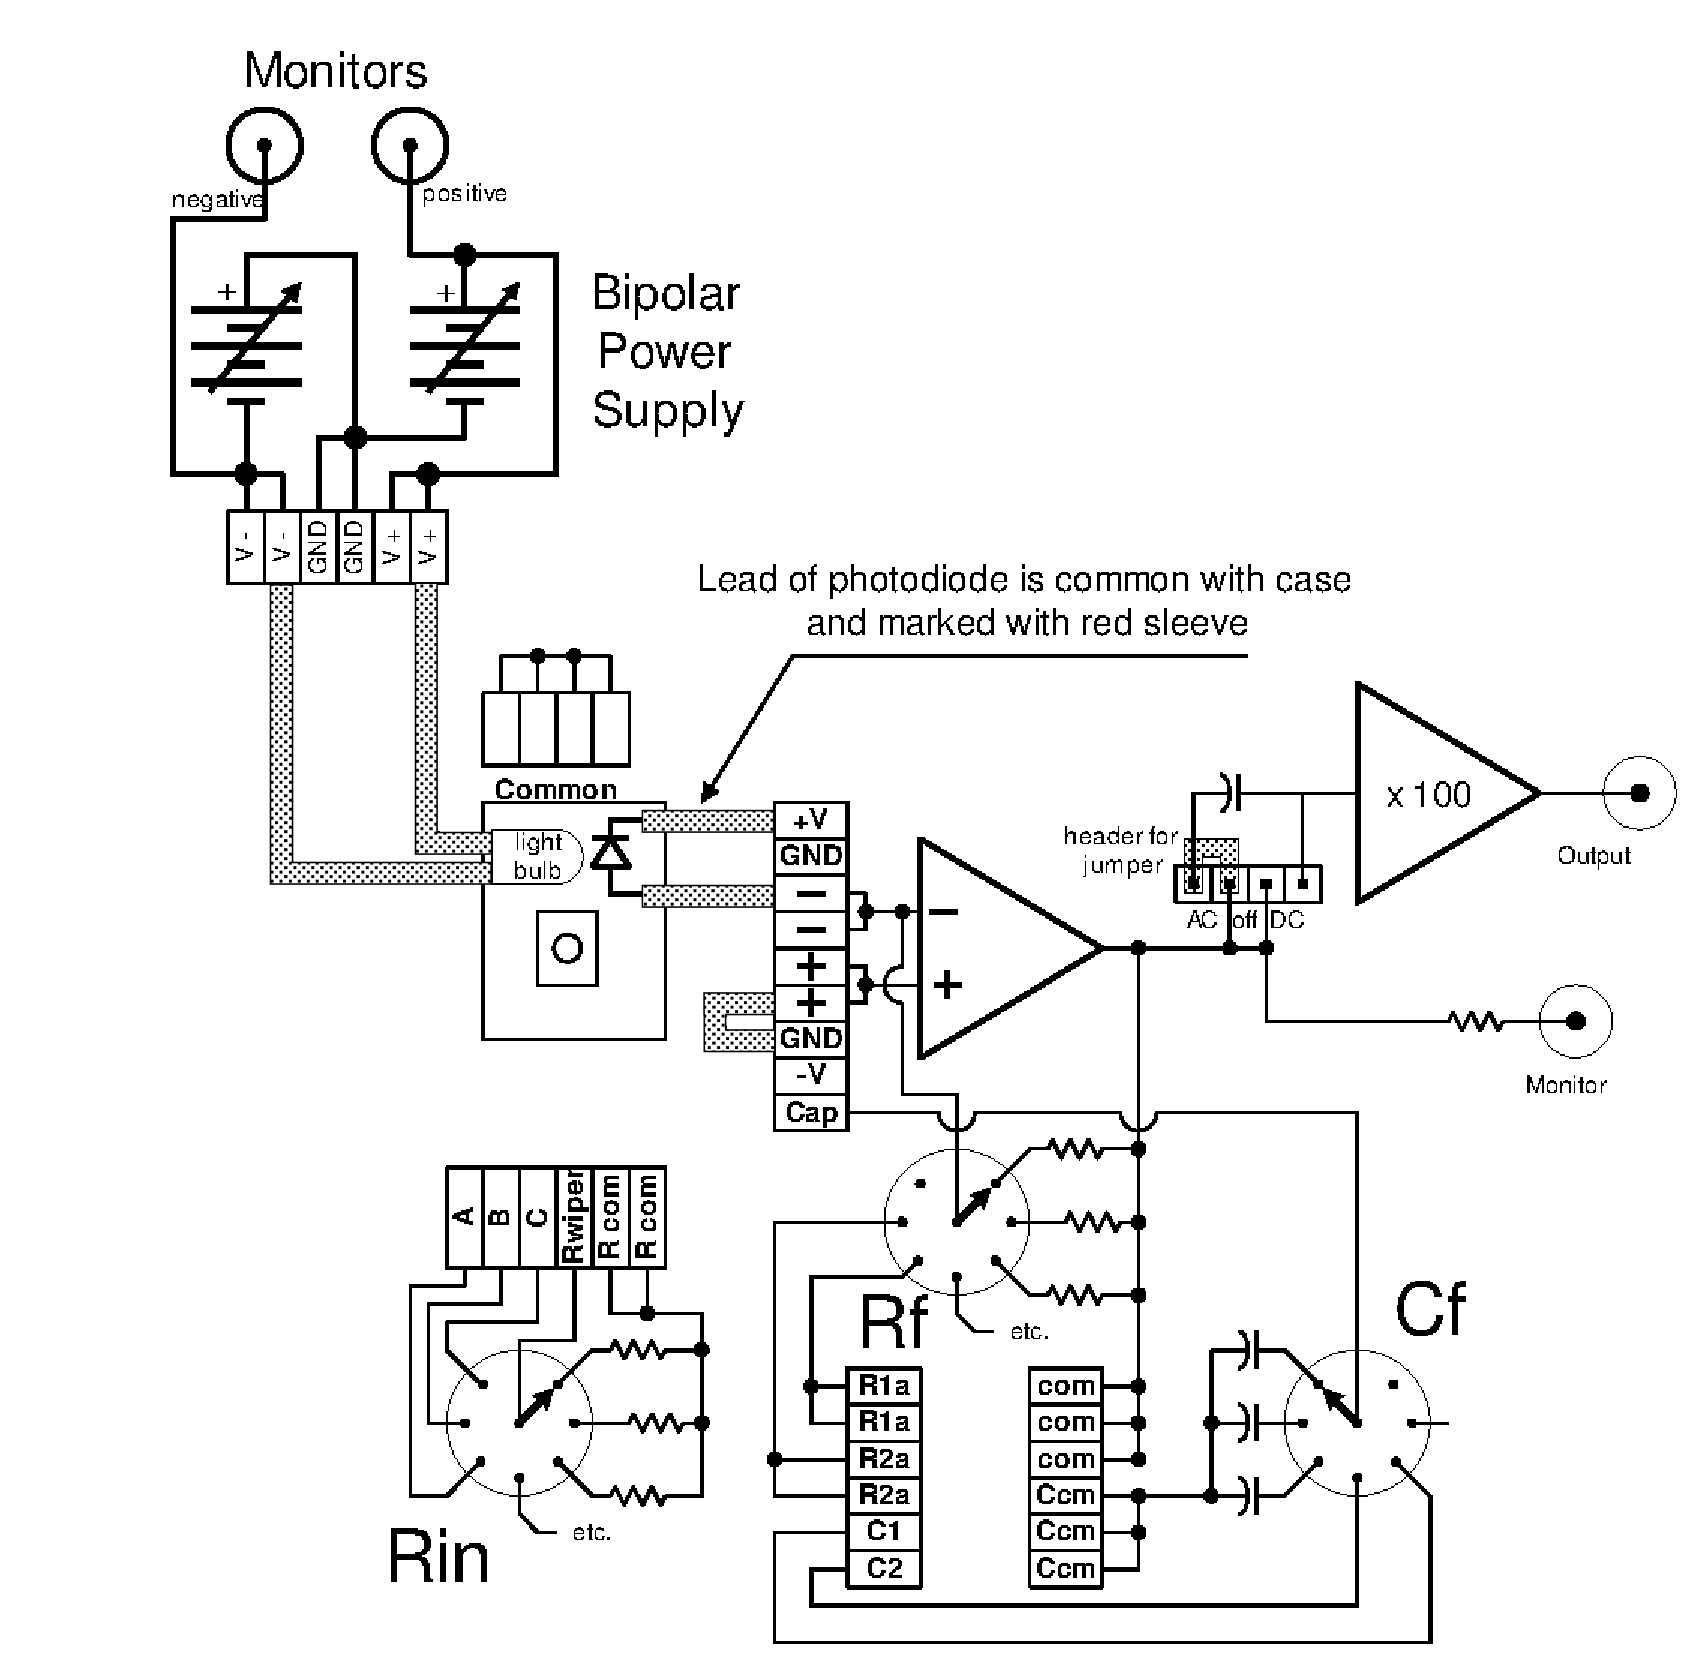
\includegraphics[width=\textwidth]{figs/schrot lle.png}
        \caption{LLE-Box: Verstärkung des Photostroms}
        \label{fig:schrotlle}
    \end{subfigure}
    \hfill
    \begin{subfigure}[t]{0.48\textwidth}
        \centering
        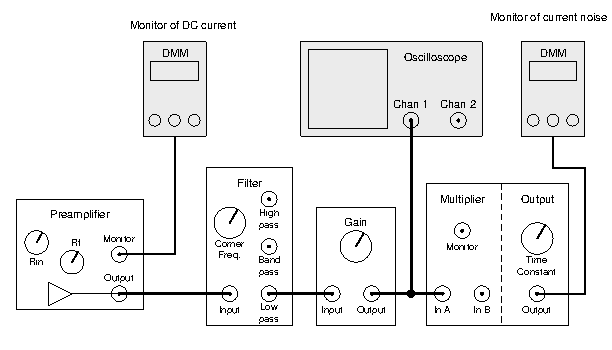
\includegraphics[width=\textwidth]{figs/schrot hle.png}
        \caption{HLE-Box: Quadratur-Mittelwertbildung}
        \label{fig:schrothle}
    \end{subfigure}
    \caption{Signalverarbeitung zur Messung des Schrotrauschens: (a) LLE-Box, (b) HLE-Box \cite{praktikum}}
    \label{fig:schrotboxes}
\end{figure}
\FloatBarrier

Die weitere Signalverarbeitung erfolgt über die HLE-Box  (Abb. \ref{fig:schrotboxes}b). 
Der integrierte Multiplizierer arbeitet im AxA-Modus und berechnet den quadratischen Mittelwert der Eingangsspannung:

\begin{equation}
    V_{\text{out}} = \frac{V(t)^2}{10 \, \si{V}}
\end{equation}

Nach zeitlicher Mittelung ergibt sich das Ausgangssignal der HLE-Box \( V_{\text{meter}} \), das proportional zur mittleren Stromschwankung ist:

\begin{equation}
    \overline{\delta i^2} = \frac{\overline{V_{\text{meter}}} \cdot 10 \, \si{V}}{(100 \cdot G_2 \cdot R_f)^2}, \qquad 
    \Delta\overline{\delta i^2} = \frac{\Delta \overline{V_{\text{meter}}} \cdot 10 \, \si{V}}{(100 \cdot G_2 \cdot R_f)^2}
\end{equation}

Zur Messung des Schrotrauschens wird der Tiefpass der HLE-Box auf eine Grenzfrequenz von \( f_{\text{gr}} = \SI{100}{\kilo\hertz} \) eingestellt, alle Schalter stehen auf AC-Kopplung. 
Die Verstärkung \( G_2 \) wird so gewählt, dass das Signal \( \overline{V_{\text{meter}}} \) im Bereich von etwa \( 0{.}6\,\si{V} \) bis \( 1{.}2\,\si{V} \) liegt, um im linearen Messbereich zu bleiben.

\subsection{Untergrundbeiträge}

Um sicherzustellen, dass die Messungen unbeeinflusst - also ohne äußere Störeinflüsse - durchgeführt werden können, müssen potenzielle externe Einflüsse dokumentiert werden. Zu diesem Zweck wird die Lampenspannung abgeschaltet (auf Null gesetzt) und der Regler \( G_2 \) auf den Wert 6000 eingestellt.

Dabei ergibt sich eine gemessene Spannung von
\begin{equation*}
    V_{\text{meter},0} = \SI{1.058 \pm 0.008}{\volt}.
\end{equation*}
Daraus ergibt sich eine effektive Rauschleistung (RMS-Offset):
\begin{equation*}
    \overline{\delta i_{offset}^2} = (2{.}94 \pm 0{.}02) \times 10^{-19} \si{A^2}.
\end{equation*}
Da der gemessene Fehler nicht ausschließlich durch die HRE-Box verursacht wird, sondern auch durch den Vorverstärker, wird zusätzlich die Vorverstärker Spannung an einer abgeschalteten Glühlampe gemessen. 
Dies ist notwendig, da ein eventueller Gleichstromanteil \( i_{\text{dc}} \) das Messergebnis verfälschen kann. 
Die gemessene Spannung beträgt:
\begin{equation*}
    V_{\text{monitor},0} = (-0.4 \pm 0.1) \si{\milli\volt}.
\end{equation*}

Zusätzlich besteht die Möglichkeit, dass das Multimeter am Monitor-Ausgang des Vorverstärkers das Rauschniveau des Multimeters am Ausgang der HRE-Box beeinflusst. 
Um diesen Effekt zu untersuchen, wurde das Multimeter am Vorverstärker mehrfach an- und abgesteckt. Die resultierenden Messwerte von \( V_{\text{meter}} \) zeigen eine geringe Abweichung, die jedoch innerhalb des statistischen Fehlers (\(1\sigma\)) liegt.
Somit kann dieser Einfluss als vernachlässigbar angesehen werden.

\subsection{Abhängigkeit des Schrotrauschen vom Gleichstrom}

Damit die Abhängigkeit des Schrotrauschens vom Gleichstrom untersucht werden kann, werden die Ausgangsspannungen \(V_{\text{monitor}}\) und \(V_{\text{meter}}\) für unterschiedliche Glühbirnenspannungen gemessen. 
Die Messwerte sind in Tabelle \ref{tab:Schrot_Gleichstrom} dargestellt.

\begin{table}[H]
    \centering
    \begin{tabular}{c|c|c}
        Gain & \(-V_{\text{monitor}}~[\text{V}]\) & \(V_{\text{meter}}~[\text{V}]\) \\
        \hline
        6000 & 0.0004 \(\pm\) 0.0001 & 1.058 \(\pm\) 0.008 \\
        5000 & 0.0119 \(\pm\) 0.0001 & 0.848 \(\pm\) 0.006 \\
        5000 & 0.0161 \(\pm\) 0.0001 & 0.886 \(\pm\) 0.006 \\
        1500 & 1.255 \(\pm\) 0.001 & 1.169 \(\pm\) 0.004 \\
        1000 & 1.641 \(\pm\) 0.001 & 0.686 \(\pm\) 0.004 \\
        1000 & 2.181 \(\pm\) 0.001 & 0.912 \(\pm\) 0.004 \\
        800 & 3.602 \(\pm\) 0.01 & 0.963 \(\pm\) 0.004 \\
        600 & 4.74 \(\pm\) 0.01 & 0.733 \(\pm\) 0.006 \\
        600 & 5.55 \(\pm\) 0.01 & 0.860 \(\pm\) 0.004 \\
        600 & 6.16 \(\pm\) 0.01 & 1.000 \(\pm\) 0.004 \\
        600 & 7.13 \(\pm\) 0.01 & 1.110 \(\pm\) 0.004 \\
        500 & 9.26 \(\pm\) 0.01 & 1.008 \(\pm\) 0.004 \\
        400 & 9.66 \(\pm\) 0.01 & 0.673 \(\pm\) 0.004 \\
        400 & 10.13 \(\pm\) 0.01 & 0.736 \(\pm\) 0.004 \\
        400 & 11.04 \(\pm\) 0.01 & 0.772 \(\pm\) 0.004 \\
    \end{tabular}
    \caption{Messung der Abhängigkeit des Schrotrauschens vom Gleichstrom}
    \label{tab:Schrot_Gleichstrom}
\end{table}


Zur Berücksichtigung des Untergrundrauschens werden die korrigierten Gleichströme und Rauschleistungen über folgende Gleichungen berechnet:
\begin{equation}
    i_{\text{dc,korr}} = \frac{-(V_{\text{monitor}} - V_{\text{monitor},0})}{R_f}, \qquad 
    \Delta i_{\text{dc,korr}} = \sqrt{\left(\frac{\Delta V_{\text{monitor}}}{R_f}\right)^2 + \left(\frac{\Delta V_{\text{monitor},0}}{R_f}\right)^2}
\end{equation}
\begin{equation}
    \overline{\delta i_{\text{korr}}^2} = \frac{\overline{V_{\text{meter}}(t)} \cdot 10~\text{V}}{(100 \cdot G_2 R_f)^2} - \overline{\delta i_{\text{offset}}^2}, \qquad 
    \Delta \overline{\delta i_{\text{korr}}^2} = \sqrt{\left(\frac{\Delta V_{\text{meter}} \cdot 10~\text{V}}{(100 \cdot G_2 R_f)^2}\right)^2 + \left(\Delta \overline{\delta i_{\text{offset}}^2}\right)^2}
\end{equation}

Die resultierenden Werte sind in Tabelle \ref{tab:Schrotg} aufgeführt.

\FloatBarrier
\begin{table}[]
    \centering
    \begin{tabular}{c|c}
        \(-i_{\text{dc,korr}}\, [\text{A}]\) & \(\overline{\delta i_{\text{korr}}^2}\, [\text{A}^2]\) \\
        \hline
        \((0.00 \pm 1.00) \times 10^{-8}\) & \((-0.11 \pm 3.14) \times 10^{-21}\) \\
        \((1.15 \pm 0.01) \times 10^{-6}\) & \((4.52 \pm 0.39) \times 10^{-20}\) \\
        \((1.57 \pm 0.01) \times 10^{-6}\) & \((6.04 \pm 0.39) \times 10^{-20}\) \\
        \((12.55 \pm 0.01) \times 10^{-5}\) & \((4.90 \pm 0.03) \times 10^{-18}\) \\
        \((16.41 \pm 0.01) \times 10^{-5}\) & \((6.57 \pm 0.06) \times 10^{-18}\) \\
        \((21.81 \pm 0.01) \times 10^{-5}\) & \((8.83 \pm 0.06) \times 10^{-18}\) \\
        \((36.02 \pm 0.01) \times 10^{-5}\) & \((14.75 \pm 0.06) \times 10^{-18}\) \\
        \((4.74 \pm 0.01) \times 10^{-4}\)  & \((2.01 \pm 0.02) \times 10^{-17}\) \\
        \((5.55 \pm 0.01) \times 10^{-4}\)  & \((2.36 \pm 0.01) \times 10^{-17}\) \\
        \((6.16 \pm 0.01)\times 10^{-4}\)  & \((2.75 \pm 0.01) \times 10^{-17}\) \\
        \((7.13 \pm 0.01) \times 10^{-4}\)  & \((3.05 \pm 0.01) \times 10^{-17}\) \\
        \((9.26 \pm 0.01) \times 10^{-4}\)  & \((4.00 \pm 0.02) \times 10^{-17}\) \\
        \((9.66 \pm 0.01) \times 10^{-4}\)  & \((4.18 \pm 0.02)\times 10^{-17}\) \\
        \((10.13 \pm 0.01) \times 10^{-4}\) & \((4.57 \pm 0.02) \times 10^{-17}\) \\
        \((11.04 \pm 0.01) \times10^{-4}\) & \((4.80 \pm 0.02)\times 10^{-17}\) \\
        
    \end{tabular}
    \caption{Berechnete korrigierte Ströme und Rauschleistungen}
    \label{tab:Schrotg}
\end{table}
\FloatBarrier

Die dargestellten Werte wurden in Abbildung \ref{fig:schrotgleich} grafisch aufgetragen. Der Zusammenhang lässt sich durch eine lineare Beziehung der Form \(y(x) = a \cdot x + b\) beschreiben, wobei sich für die Steigung ergibt:
\begin{equation*}
    a = (-4.278 \pm 0.322) \times 10^{-14}~\si{\frac{A^2}{A}} 
\end{equation*}
\begin{equation*}
    b = (-0.068 \pm 1.082) \times 10^{-19} \si{A}^2
\end{equation*}

\begin{figure}[htbp]
    \centering
    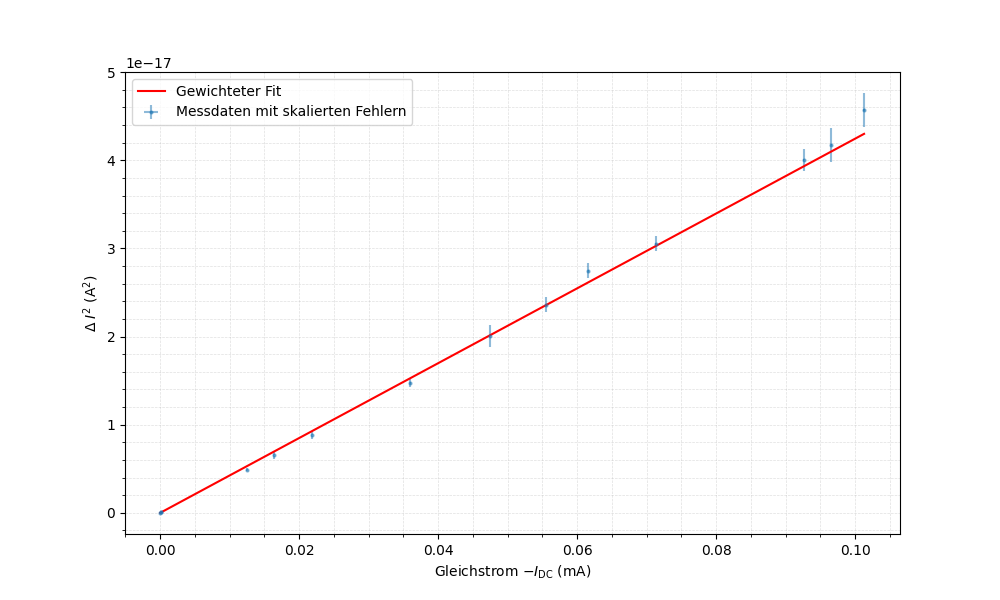
\includegraphics[width=1\textwidth]{figs/schrotgleich_5.png}
    \caption{Mittlere quadratische Stromfluktuation in Abhängigkeit vom korrigierten Gleichstrom. \(\chi^2 = 56.20\). Werte aus Tabelle \ref{tab:Schrotg}.}
    \label{fig:schrotgleich}
\end{figure}


Der deutlich erhöhte \(\chi^2\) -Wert lässt vermuten, dass die Unsicherheiten der Messwerte zu niedrig angesetzt wurden. Eine realistischere Fehlerabschätzung würde 

Die beobachtete Abweichung könnte durch zusätzliche Rauschanteile verursacht worden sein, die bei der Auswertung als vernachlässigbar angenommen wurden. Hierzu zählen insbesondere thermisches Rauschen, das bei zu langen Integrationszeiten verstärkt auftritt, sowie kurzzeitige Fluktuationen, etwa durch Netzstörungen oder Drift in der Verstärkerelektronik. 

Darüber hinaus könnten systematische Abweichungen durch eine ungenaue Kalibrierung des Verstärkersystems entstanden sein. Besonders kritisch ist hierbei die Bestimmung des Verstärkungsfaktors \textit{Gain}, da dieser quadratisch in die Berechnung von $\Delta I^2$ eingeht und somit kleine Kalibrierfehler einen großen Einfluss auf das Endergebnis haben können.


\subsection{Abhängigkeit des Schrotrauschens von der Bandbreite}

Es wurde nun der Gleichstrom und Aufbau, Gleichgehalten, damit die "Weißheit" der Schrotrauschen überprüft werden kann.
Somit ist:
\begin{equation*}
    V_{monitor} = (-6.67 \pm 0.02) \si{\volt}
\end{equation*}

Dabei wird die Verstärkung so geändert, dass die Ausgangsannung der HLE-Box -\(V_{meter}\)- in Bereich zwischen 0.6 V und 1.2 V liegt. 
Diese Messwerte inklusieve Berechneten Werte sind in Tabelle \ref{tab:schrotbreite} aufgelistet, mit ein Widerstand \(R_f = 10\)kHz. 

\begin{table}[H]
    \centering
    \begin{tabular}{c|c|c|c|c}
        \(f_l\) [Hz] & \(G_2\) & \(V_{meter}\)[V] & \(\Delta f\)[Hz] & \(\overline{\delta i_{korr}^2}[\text{A}^2]\) \\
        \hline
        330 & 10000 & 0.740 \(\pm\) 0.010 & 366.54 & (-2.20 \(\pm\) 0.02) \(\times 10^{-19}\) \\
        1000 & 6000 & 0.857 \(\pm\) 0.006 & 1110.72 & (-5.59 \(\pm\) 0.28) \(\times 10^{-20}\) \\
        3300 & 3000 & 0.730 \(\pm\) 0.004 & 3665.38 & (5.17 \(\pm\) 0.05) \(\times 10^{-19}\) \\
        10000 & 2000& 0.992 \(\pm\) 0.004 & 11107.21 & (2.19 \(\pm\) 0.01) \(\times 10^{-18}\) \\
        33000 & 1000 & 0.899 \(\pm\) 0.004 & 36653.78 & (8.70 \(\pm\) 0.04) \(\times 10^{-18}\) \\
        100000 & 600 & 1.040 \(\pm\) 0.004 & 111072.04 & (2.86 \(\pm\) 0.01) \(\times 10^{-17}\)
    \end{tabular}
    \caption{Messung zur Abhängigkeit des Schrotrauschens von \(\Delta f\)}
    \label{tab:schrotbreite}
\end{table}

Aus diese Werten von Tab. \ref{tab:schrotbreite} kann ein Plot Abb. \ref{fig:schrotbraite} aufgespannt werden. 
Der Zusammenhang der Daten kann durch eine Lineare Gleichung \(y(x) = a \cdot x +b\) gezeigt werden. 
Diese Werte sind:
\begin{equation*}
    a = (2.414 \pm 0.080) \times 10^{-22} \frac{\text{A}^2}{\text{A}}
\end{equation*}
\begin{equation*}
    b = (-3.255 \pm 0.261) \times 10^{-19} \text{A}^2
\end{equation*}
\FloatBarrier
\begin{figure} [htbp]
    \centering
    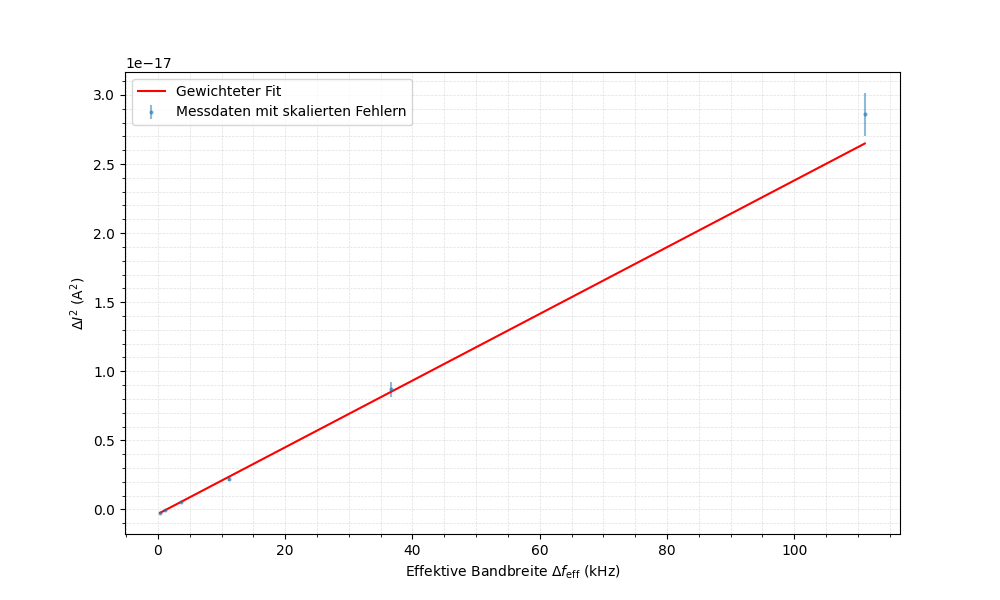
\includegraphics[width=1\linewidth]{Schrotbraite_0}
    \caption{Abhängigkeit des Schrotrauschens von der Bandbreite.\(\chi^2 = 193.56\). Werte aus Tabelle \ref{tab:schrotbreite}.}
    \label{fig:schrotbraite}
\end{figure}
\FloatBarrier
Der $\chi^2$-Wert ist hier viel größer und weist darauf hin das es zusätzlich bei dem Tiefpass ein eine ungenaue Kalibrierung aufweisen könnte.


\subsection{Berechnen der Elementarladung}

Die Elementarladung \(e\) kann anhand der Steigung der gemessenen Stromrauschleistung gemäß der Schottky-Gleichung bestimmt werden. 
Dabei gilt:

\begin{equation}
    \overline{\delta i_{\text{korr}}^2} = 2 e i_{\text{dc,korr}} \Delta f,
\end{equation}

woraus sich der experimentelle Wert der Elementarladung für verschiedene Messansätze ergibt:

\begin{equation*}
    e_{\text{exp},i} = \frac{\overline{\delta i_{\text{korr}}^2}}{2 i_{\text{dc,korr}} \Delta f} \quad \Rightarrow \quad 
    e_{\text{exp,strom}} = \frac{a}{2 \Delta f}
\end{equation*}

wobei \(i\) entweder den Gleichstrom oder die Bandbreite repräsentiert. Entsprechend kann man auch schreiben:

\begin{equation*}
    e_{\text{exp,strom}} = \frac{a}{2 \Delta f} \quad \text{bzw.} \quad e_{\text{exp,freq}} = \frac{a}{2 i_{\text{dc,korr}}}.
\end{equation*}

Die effektive Bandbreite \(\Delta f\) für den Gleichstrom ergibt sich aus dem Frequenzintegral

\begin{equation}
    \Delta f = \int_0^{\infty} \frac{1}{1+\left(\frac{f}{f_l}\right)^4} \, \mathrm{d}f = 111{,}07\,\si{kHz}.
\end{equation}

Aus den Messwerten ergeben sich folgende experimentelle Werte für die Elementarladung:

\begin{align}
    e_{\text{exp,strom}} &= (1{,}914 \pm 0{,}021) \cdot 10^{-19}~\si{C}, \\
    e_{\text{exp,freq}} &= (1{,}809 \pm 0{,}060) \cdot 10^{-19}~\si{C}.
\end{align}

Die beiden Werte unterscheiden sich merklich voneinander, was darauf hindeutet, dass die Änderung der Glühbirnenspannung einen größeren Einfluss auf zusätzliche Rauschanteile haben könnte als ursprünglich angenommen.

Zum Vergleich beträgt der Literaturwert der Elementarladung \cite{codata}:

\begin{equation}
    e_{\text{lit}} = 1{,}602176634 \cdot 10^{-19}~\si{C}.
\end{equation}

Die Abweichungen der experimentellen Werte vom Literaturwert sind signifikant: Der Wert, der aus der Frequenzvariation bestimmt wurde, liegt in etwa im 5-\(\sigma\)-Bereich, während der aus der Gleichstromvariation ermittelte Wert etwa 15 \(\sigma\) vom Literaturwert entfernt ist. Dies spricht dafür, dass vor allem die Änderung der Glühbirnenspannung und damit des Gleichstroms einen wesentlichen Einfluss auf das Messergebnis hat. Möglicherweise trägt die Glühlampe selbst als nicht vollständig ausgeschaltete Störquelle zum Rauschen bei, wodurch die Messung systematisch verfälscht wird.

Nichtsdestotrotz liegen beide experimentellen Werte in der gleichen Größenordnung und bestätigen somit grundsätzlich die Anwendbarkeit der Messmethode zur Bestimmung der Elementarladung.